\section{Numerical Experiments}\label{sec:experiments}
The aim of this section is twofold.
In Section~\ref{sec:synthetic}, we study a synthetic example that matches our theoretical assumptions and show that DP-SGD attains dimension-independent empirical and population loss when the sequence of restricted Lipschitz coefficients decays rapidly---even when gradients span the entire ambient space.
In Section~\ref{sec:lm}, we study a stylized example of privately fine-tuning large language models. 
Building on the previous theory, we provide insights as to why dense fine-tuning can yield good performance. 

\subsection{Synthetic Example: Estimating the Generalized Geometric Median}\label{sec:synthetic}
We privately estimate the geometric median which minimizes the average Mahalanobis distance. 
Specifically, let $x_i \in \R^d$ for $i \in [n]$ be feature vectors drawn i.i.d. from some distribution $P_x$, each of which is treated as an individual record. 
Denote the entire dataset as $\mathcal{D} = \{ x_i\}_{i=1}^n$.
Subject to differential privacy, we perform the following optimization
\eq{\label{eq:synth}
\min_{ x \in \R^d} F_\alpha (x)
	=
		\frac{1}{n} \sum_{i=1}^n f_i (x) + \frac{\alpha}{2} \normtwo{ x - x^{(0)} }^2
	= 
		\frac{1}{n} \sum_{i=1}^n \left\| x - x_i \right\|_A  + \frac{\alpha}{2} \normtwo{ x - x^{(0)} }^2,
}
where we adopt the shorthand $f_i(x) = f(x; x_i) = \norm{x - x_i}_A$.
When $A = I_d$ and $\alpha=0$ (without the regularization term), the problem reduces to estimating the usual geometric median (commonly known as center of mass). 

For this example, individual gradients are bounded since $\| \nabla f_i( x ) \|_2 = \| A (x - x_i)  / \| x - x_i \|_A \|_2 \le \lambda_1(A^{1/2}) = G_0$.
More generally, the restricted Lipschitz coefficients of $F(x)$ are the eigenvalues of $A^{1/2}$, since 
\eqn{
	\| Q_k \nabla F(x) \|_2
=
	 \left\|Q_k A^{1/2} \frac{1}{n} \sum_{i=1}^n \frac{ A^{1/2}( x - x_i ) }{ \| x - x_i \|_A } \right\|_2
\le
	\| Q_k A^{1/2} \|_\text{op} = \lambda_{k+1}(A^{1/2}) = G_k, 
}
where $Q_k = I - P_k$ is chosen to be the rank $(d-k)$ orthogonal projection matrix that projects onto the subspace spanned by the bottom $(d-k)$ eigenvectors of $A^{1/2}$.

To verify our theory, we study the optimization and generalization performance of DP-SGD for minimizing~\eqref{eq:synth} under Mahalanobis distances induced by different $A$ as the problem dimension grows. 
The optimization performance is measured by the final training error, and the generalization performance is measured by the population quantity $\mathbb{E}_{x \sim P_x, \ox} [ \| \ox - x \|_A ]$, where $\ox$ denotes the random output of DP-SGD.
We study the dimension scaling behavior for $A$ being one of 
\eqn{
A_{\text{const}} = \text{diag}( 1, \dots, 1 ), \;\;
A_{\text{sqrt}} = \text{diag}( 1, 1 / \sqrt{2}, \dots, 1 / \sqrt{d} ), \;\; 
A_{\text{linear}} = \text{diag} ( 1, 1 / 2, \dots, 1 / d ),
}
where $\text{diag}: \R^d \to \R^{d \times d}$ maps vectors onto square matrices with inputs on the diagonal.
In all cases, the span of gradients $\text{span}( \{ \nabla F(x) \} )$ is the ambient space $\R^d$, since $A$ is of full rank.
To ensure the distance from the initial iterate $\beta^{(0)} = 0$ to the optimum is the same for problem instances of different dimensions, we let feature vectors $\{x_i\}_{i=1}^n$ take zero values in any dimension $k > d_{\text{min}}$, where $d_{\text{min}}$ is the dimension of the smallest problem in our experiments.
Our theoretical bounds suggest that when the sequence of restricted Lipschitz coefficients is constant (when $A = A_{\text{const}}$), the excess empirical loss grows with the problem dimension, whereas when the sequence of $k$th-Lipschitz constants rapidly decays with $k$ (when $A = A_{\text{sqrt}}$ or $A = A_{\text{linear}}$), the excess empirical loss does not grow beyond a certain problem dimension. 
Figure~\ref{fig:toy} empirically captures this phenomenon. 
We include additional experimental setup details in Appendix~\ref{app:exp_synth}.
\begin{figure}[t]
\begin{center}
\begin{minipage}[t]{0.48\linewidth}
\centering
{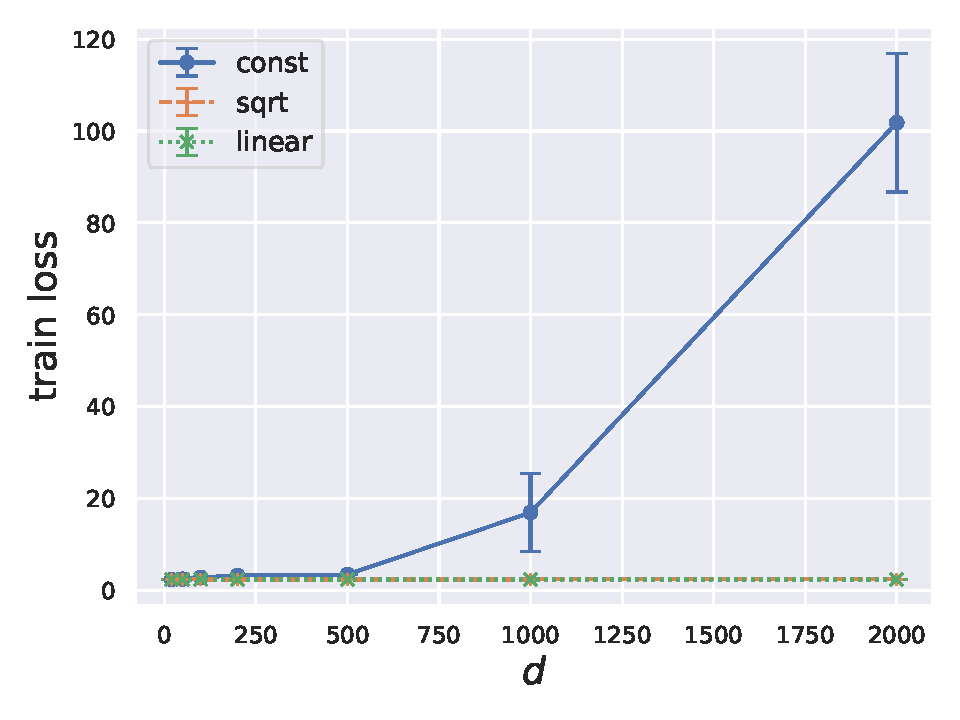
\includegraphics[width=0.98\textwidth]{figs/synthetic/trplot.pdf}}
(a) empirical loss
\end{minipage}
\begin{minipage}[t]{0.48\linewidth}
\centering
{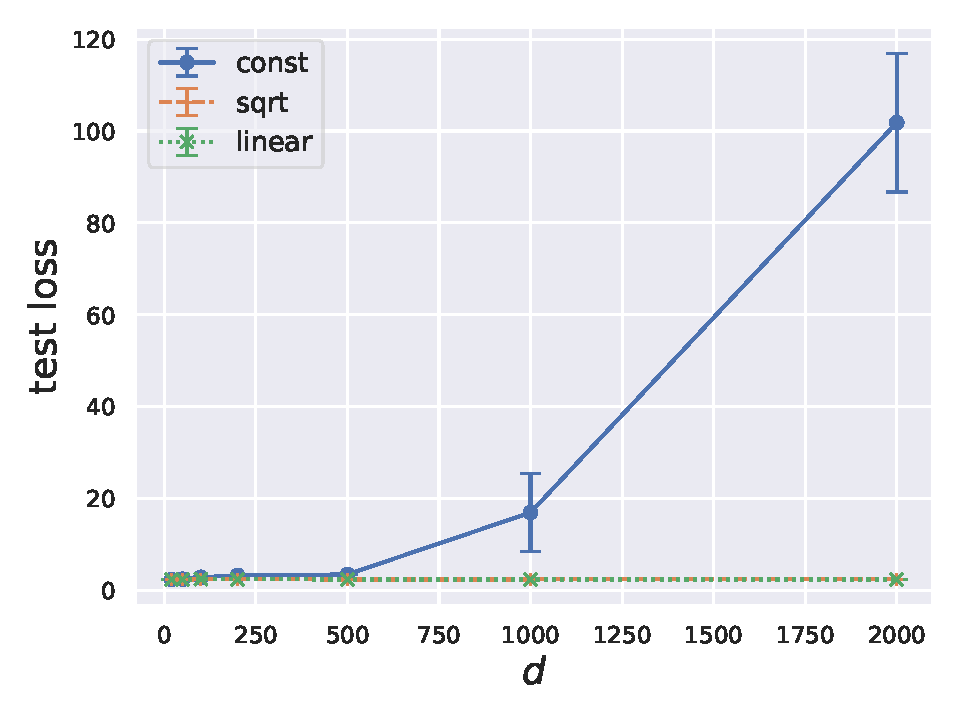
\includegraphics[width=0.98\textwidth]{figs/synthetic/teplot.pdf}}
(b) (estimated) population loss
\end{minipage}
\end{center}
\caption{
The empirical and population losses grow with increasing problem dimension when the sequence of restricted Lipschitz coefficients remain constant. On the other hand, these losses remain almost constant when the sequence of restricted Lipschitz coefficients decays rapidly.
Error bars represent one standard deviation over five runs of DP-SGD with the same hyperparameters which were tuned on separate validation data.
For the same $A$, the optimal training error $\min_{x\in\R^d} F(x)$ is the same for problem instances with different dimensions (thus errors do not scale if learning was non-private).
Each training run was performed with $\epsilon=2$, $\delta=10^{-6}$, and $n=10000$. 
}
\label{fig:toy}
\end{figure}

\subsection{Why Does Dense Fine-Tuning Work Well for Pretrained Language Models?}\label{sec:lm}
Stated informally, our bounds in Theorem~\ref{thm:DPSCO} imply that DP-SGD obtains dimension-independent errors if gradients approximately reside in a subspace much smaller than the ambient space.
Inspired by these results for the convex case, we now turn to study dense language model fine-tuning~\cite{li2021large} and provide a possible explanation for their recent intriguing success --- fine-tuning gigantic parameter vectors frequently results in moderate performance drops compared to non-private learning.


In the following, we present evidence that gradients obtained through fine-tuning mostly lie in a small subspace.
We design subsequent experiments to work under a simplified setup. 
Specifically, we fine-tune DistilRoBERTa~\cite{sanh2019distilbert,liu2019roberta} under $\epsilon=8$ and $\delta = \nicefrac{1}{n^{1.1}}$ for sentiment classification on the SST-2 dataset~\cite{socher2013recursive}.
We reformulate the label prediction problem as templated text prediction~\cite{li2021large}, and fine-tune only the query and value matrices in attention layers.

We focus on fine-tuning these specific parameter matrices due to the success of LoRA for non-private learning~\cite{hu2021lora} which focuses on adapting the attention layers. Unlike LoRA, we fine-tune all parameters in these matrices rather than focusing on low-rank updates.
This gives a setup that is lightweight enough to run spectral analyses computationally tractably but retains enough parameters ($\approx7$ million) such that a problem of similar scale outside of fine-tuning results in substantial losses in utility.\footnote{For instance, an off-the-shelf ResNet image classifier has 10 to 20+ million parameters. A plethora of works report large performance drops when training these models from scratch~\cite{YZCL21,luo2021scalable,de2022unlocking}.}
For our setup, DP-SGD obtains a dev set accuracy approximately of $90\%$ and $92\%$, privately and non-privately, respectively.
These numbers are similar to previous results obtained with the same pretrained model~\cite{yu2021differentially,li2021large}. We include the full experimental protocol and additional results in Appendix~\ref{app:exp_privlm}. 

To provide evidence for the small subspace hypothesis, we sample gradients during fine-tuning and study their principal components.
Specifically, we ``over-train'' by privately fine-tuning for $r = 2 \times 10^3$ updates and collect all the non-privatized average clipped gradients along the optimization trajectory.
While fine-tuning for 200 and 2k updates have similar final dev set performance under our hyperparameters, the increased number of steps allows us to collect more gradients around the converged solution. 
This yields a gradient matrix $H \in \R^{r \times p}$, where $p \approx 7 \times 10^6$ is the size of the parameter vector. 
We perform PCA for $H$ with the orthogonal iteration algorithm~\cite{demmel1997applied} and visualize the set of estimated singular values $\sigma_i(H) = \lambda_i(H^\top H)^{1/2}$ in terms of both (i) the density estimate, and (ii) their relation with the rank.
Figure~\ref{fig:pca} (a) shows the top 1000 singular values sorted and plotted against their rank $k$ and the least squares fit on log-transformed inputs and outputs.
The plot displays few large singular values which suggests that gradients are controlled through only a few principal directions.
The linear fit suggests that singular values decay rapidly (at a rate of approximately $k^{-0.6}$).

To study the effects that different principal components have on fine-tuning performance, we further perform the following re-training experiment. 
Given the principal components, we privately re-fine-tune with gradients projected onto the top $k \in \{10, 20, 100\}$ components.
Note that this projection applies only to the (non-privatized) average clipped gradients and the isotropic DP noise is still applied to all dimensions.
Figure~\ref{fig:pca} (b) shows that the original performance can be attained by optimizing within a subspace of only dimension $k=100$, suggesting that most of the dimensions of the 7 million parameter vector encode a limited learning signal.

While these empirical results present encouraging insights for the dimension-independent performance of fine-tuning, we acknowledge that this is not a complete validation of the restricted Lipschitz continuity condition and fast decay of coefficients (even locally near the optimum).
We leave a more thorough analysis with additional model classes and fine-tuning tasks to future work.

\begin{figure}[thb]
\begin{center}
\begin{minipage}[t]{0.48\linewidth}
\centering
{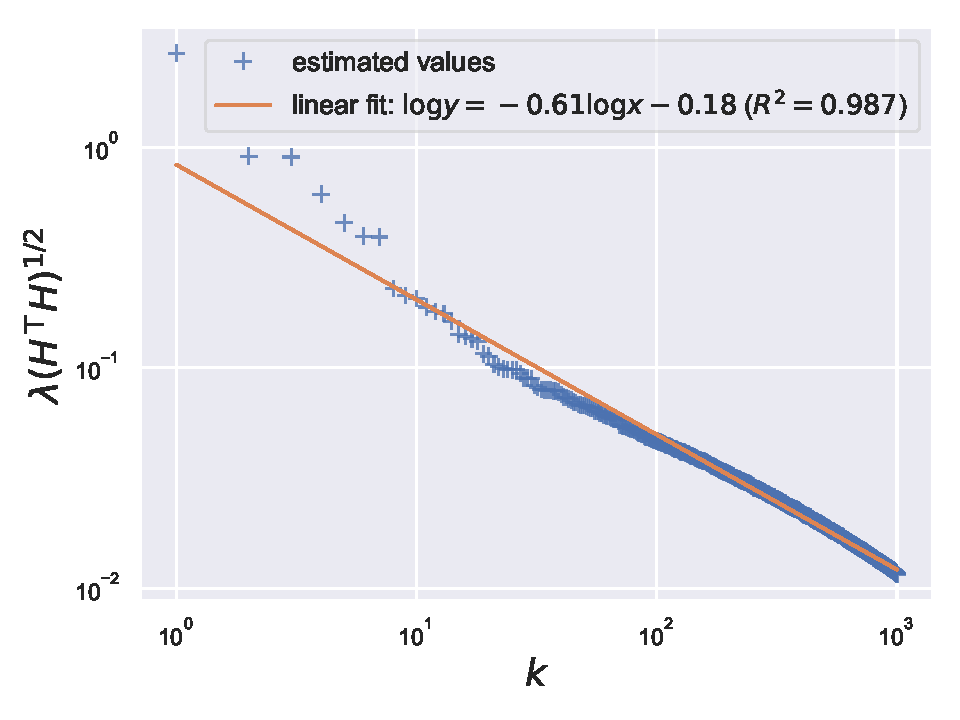
\includegraphics[width=0.98\textwidth]{figs/privlm/roberta/eigenvalue-linfit.pdf}}
\footnotesize{(a) singular values decay with rank}
\end{minipage}
\begin{minipage}[t]{0.48\linewidth}
\centering
{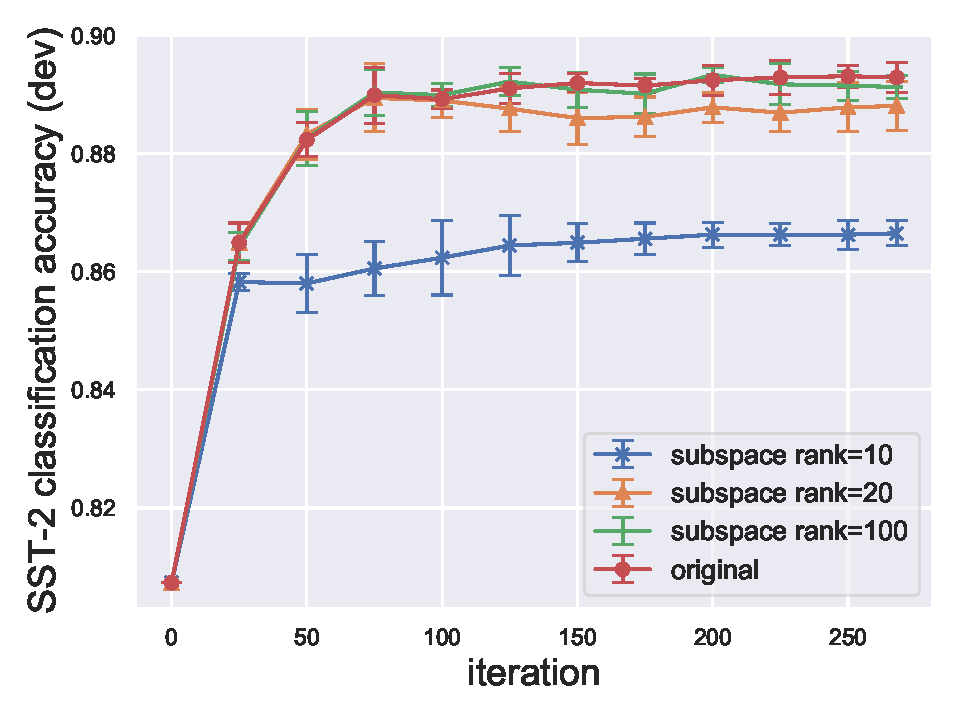
\includegraphics[width=0.98\textwidth]{figs/privlm/roberta/plot2.pdf}}
\footnotesize{(b) retrain in fixed subspace}
\end{minipage}
\end{center}
\caption{
Gradients obtained through fine-tuning are controlled by a few principal components.
\emph{Left:} Singular values decay rapidly with their rank.
\emph{Right:} Retraining with gradients projected onto a subspace (but noise is not projected!) is sufficient to recover original performance.
}
\label{fig:pca}
\end{figure}

% good performance of dense DP fine-tuning is due to gradients mostly residing in a low dimension subspace, we perform the intervention of identifying an approximation of this subspace and (re-)train with gradients explicitly projected onto this subspace.
% The projection step clears out any learning signal that is encoded in the remaining directions, and thus if fine-tuning relied heavily on those directions, one would expect large performance drops. 

% To identify the subspace, we first perform a usual DP fine-tuning round and collect all the average clipped gradients reported along the training trajectory.
% We then run PCA to extract the top principal components which define a subspace, and we perform a second round of DP fine-tuning.  
% This time, before each update, we explicitly project the average clipped gradients at each step onto our low dimensional subspace spanned by the principal components.
% Note that isotropic Gaussian noise is still applied to all coordinates before every update to ensure the DP constraint isn't violated. 
% Figure~\ref{fig:pca} shows that the second round of DP fine-tuning attains almost the same final performance as the first round of DP fine-tuning, even though gradients are projected onto a much smaller subspace.

% \begin{figure}[thb]
% \begin{center}
% \begin{minipage}[t]{0.32\linewidth}
% \centering
% {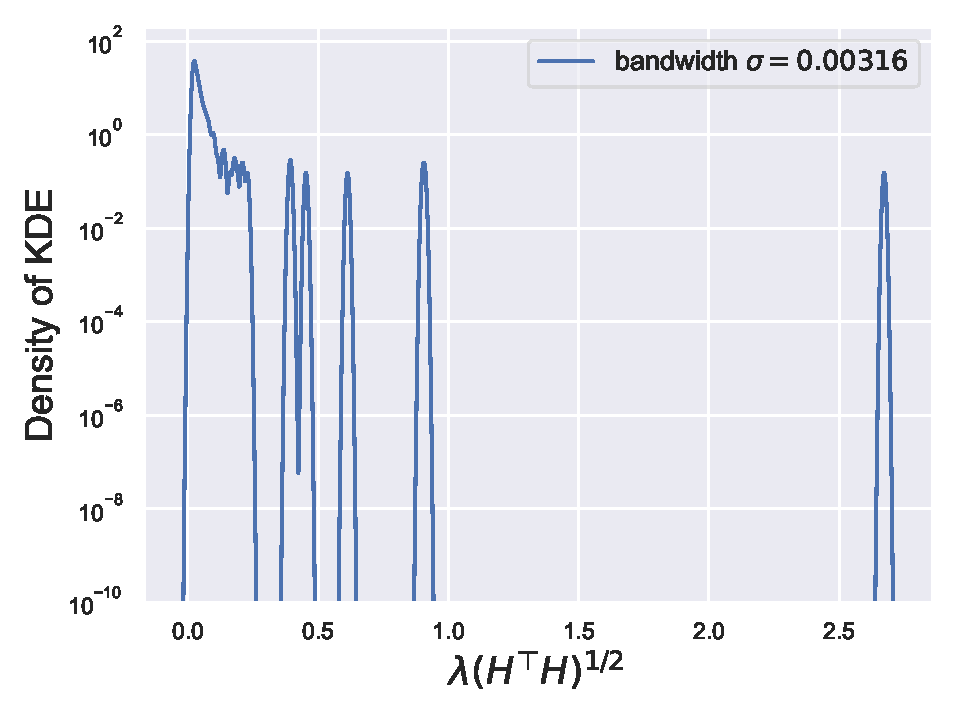
\includegraphics[width=0.98\textwidth]{figs/privlm/roberta/eigenvalue-density.pdf}} \\ \vspace{-0.10cm}
% \footnotesize{(a) density of singular values}
% \end{minipage}
% \begin{minipage}[t]{0.32\linewidth}
% \centering
% {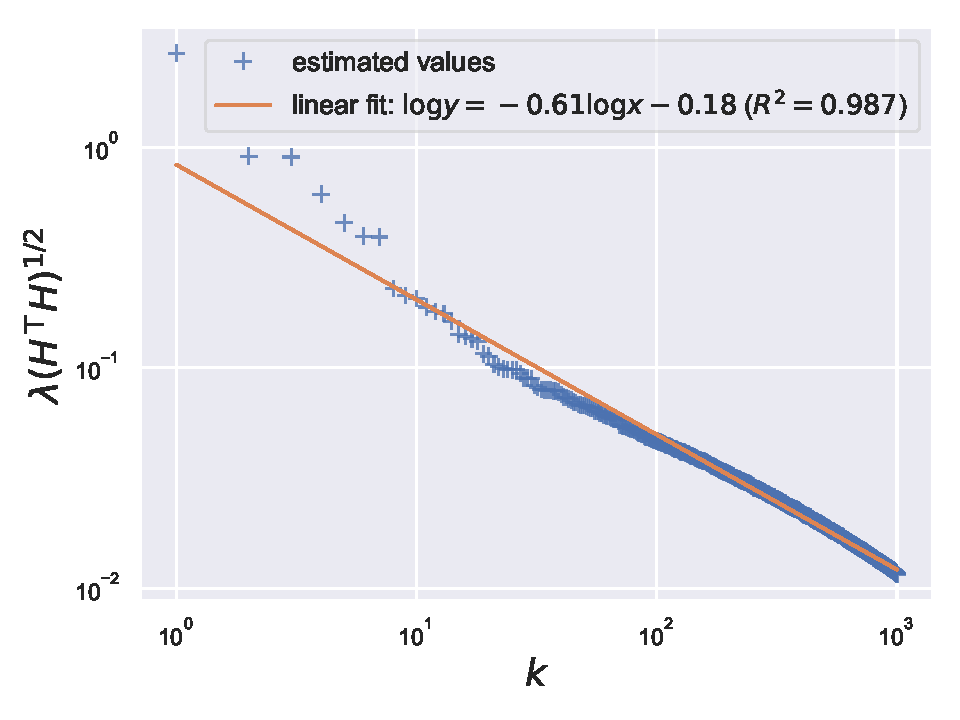
\includegraphics[width=0.98\textwidth]{figs/privlm/roberta/eigenvalue-linfit.pdf}} \\ \vspace{-0.10cm}
% \footnotesize{(b) singular values decay with rank}
% \end{minipage}
% \begin{minipage}[t]{0.32\linewidth}
% \centering
% {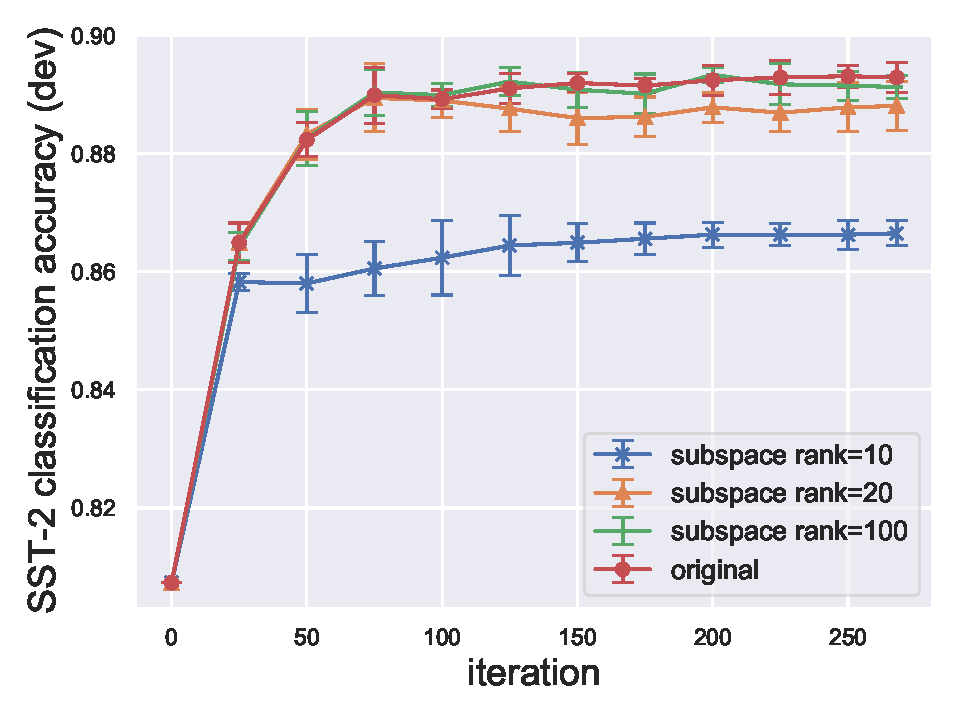
\includegraphics[width=0.98\textwidth]{figs/privlm/roberta/plot2.pdf}} \\ \vspace{-0.10cm}
% \footnotesize{(c) retrain in fixed subspace}
% \end{minipage}
% \end{center}
% \caption{}
% \label{fig:pca}
% \end{figure}

% \XL{
% - Relation to GEP. 
% - Relation to GD happens in tiny subspace paper.
% - We don't actually full fine-tune. Details.
% - Clarify low dim things and its relation with the theory (find nice ways to tie things together).
% - Rewrite the subsection title.
% - Rewrite the intro paragraph for LM fine-tuning.
% - Private and non-private perf of this model.
% }
